\section{Projet NET4104 - Réception d'un signal BLE émis par ESP32 sur
le channel
37}\label{projet-net4104---ruxe9ception-dun-signal-ble-uxe9mis-par-esp32-sur-le-channel-37}

Projet s'inscrivant dans le cours NET4104 à Télécom SudParis.
\textbf{Auteurs :} - Valentin LANTIGNY ; - Jeremy LENOIR ; - Romain
MOREAU ; - Alan VAN TRIGT.

\textbf{Encadrant :} - Rémy GRUNBLATT.

\subsection{Introduction}\label{introduction}

Dans le monde de la communication sans fil, la technologie Bluetooth Low
Energy (BLE) a gagné en popularité en raison de sa faible consommation
d'énergie et de sa large gamme d'applications. La possibilité de
reproduire la chaîne de transmission BLE pour comprendre et manipuler
les signaux émis est d'un intérêt particulier pour de nombreux domaines,
de la domotique à l'Internet des Objets.

Dans cette étude, notre objectif est de comprendre comment récupérer et
décoder un signal émis par un module ESP32 en utilisant le protocole BLE
sur le canal de publicité (channel advertising) n°37. Cette tâche peut
sembler complexe, mais en décomposant le processus en différentes étapes
et en utilisant les outils appropriés, nous pouvons explorer les
mécanismes sous-jacents de cette transmission sans fil.

Notre plan de recherche se décompose en trois grandes parties. Tout
d'abord, nous explorerons des interfaces codes hardware. Par la suite,
nous aborderons l'utilisation de GNU Radio, un logiciel de traitement du
signal et de communication, pour des analyses plus approfondies et une
manipulation avancée des signaux BLE. Enfin, nous utiliserons Python,
avec ses bibliothèques spécialisées, pour décoder le signal reçu.

Cette approche progressive nous permettra de couvrir un large éventail
d'outils et de techniques, de la programmation embarquée à la
manipulation avancée de signaux, dans le but ultime de maîtriser la
reproduction et la compréhension de la chaîne de transmission Bluetooth
Low Energy.

\section{1. Choix des technologies}\label{choix-des-technologies}

Émission/Réception BLE avec ESP32 Lors de notre exploration pour créer
une architecture client-serveur en Bluetooth Low Energy (BLE) avec
l'ESP32, nous avons identifié trois solutions potentielles. Dans cette
section, nous détaillons les avantages et les inconvénients de chacune
de ces solutions.

Arduino IDE Avantage : La liaison avec l'ESP32 est directement gérée au
sein de l'IDE, offrant ainsi une facilité d'utilisation et la
possibilité de se baser sur des exemples existants pour démarrer
rapidement.

Désavantage : Cependant, les librairies disponibles peuvent ne pas être
toujours tenues à jour, ce qui peut poser des problèmes de compatibilité
avec les versions plus récentes de l'ESP32 ou avec d'autres composants.

Micropython Avantage : Micropython offre la possibilité de travailler
avec Python, un langage largement utilisé et apprécié pour sa simplicité
et sa lisibilité. Cela peut faciliter le développement et la maintenance
du code pour certains utilisateurs.

Désavantage : Cependant, l'utilisation de Micropython demande un travail
de préparation assez conséquent, notamment en ce qui concerne
l'importation de la librairie Micropython sur l'ESP32, ce qui peut
ajouter une étape supplémentaire dans le processus de développement.

ESP-IDF Avantage : L'ESP-IDF (Espressif IoT Development Framework) est
la solution native pour le développement sur les microcontrôleurs ESP32,
offrant ainsi une compatibilité et une intégration optimales avec les
fonctionnalités matérielles de ces dispositifs. De plus, en tant que
version officielle, elle est souvent la plus à jour.

Désavantage : Cependant, la programmation en C, utilisée dans l'ESP-IDF,
peut être considérée comme plus complexe pour certains développeurs
habitués à des langages de haut niveau comme Arduino ou Python.

\subsubsection{2. GNU Radio}\label{gnu-radio}

\includesvg{https://www.gnuradio.org/gnuradio_logo_glyphs_as_paths.svg}

Pour recevoir un signal Bluetooth Low Energy, la première étape va être
de recevoir et démoduler les données. Pour ce faire, une antenne
connectée à un HackRF comportant un oscillateur intégré (40 MHz) va
permettre la bonne réception du signal et l'outil GNU Radio permettra
d'effectuer la démodulation pour obtenir les données transmises.

Pour les caractéristiques techniques, la documentation
\texttt{Bluetooth\ Core\ Specification\ v5.3}\footnote{Ressources
  Bluetooth:
  https://www.bluetooth.com/specifications/specs/core-specification-5-3/}
est utilisé comme référence. Dans le cadre du projet, seul le
\texttt{canal\ 37\ Advertising} sera étudié pour simplifier les
démarches, celui-ci étant à la fréquence \(f = 2.402 \ GHz\). Le BLE
utilisé également 40 canaux de 2 MHz de large, il faudra donc une
fréquence d'échantillonnage \(f_{e} = 4 MHz\) pour satisfaire le
théorème de Nyquist-Shannon.

Le HackRF \footnote{HackRF: https://greatscottgadgets.com/hackrf/one/}
est un émetteur - récepteur de la marque Great Scott Gadgets opérant de
1 MHz à 6 GHz. Comme plusieurs systèmes d'échantillonnage en quadrature,
il peut présenter un \emph{DC Offset} : c'est un pic au centre du
spectre causé par un biais interne. Pour faire face à ce problème, le
choix retenu est de régler le HackRF sur une fréquence \(f + \delta f\)
puis d'effectuer un décalage fréquentiel de \(-\delta f\) pour revenir
au cadre d'étude \footnote{DC offset :
  https://hackrf.readthedocs.io/en/latest/faq.html\#bigspike.}, ici, il
sera fixé à \(\delta f = 1.5 \ MHz\). Par ailleurs, les données sont au
format I/Q (type \emph{complex - float32}).

Le logiciel GNU Radio permet de traiter le signal, notamment pour
moduler et démoduler. Deux types de données seront utilisés : les
\emph{complex Float 32} en sortie du HackRF, et des \emph{bytes} après
démodulation.

\textbf{Réception et filtrage}

\begin{figure}
\centering
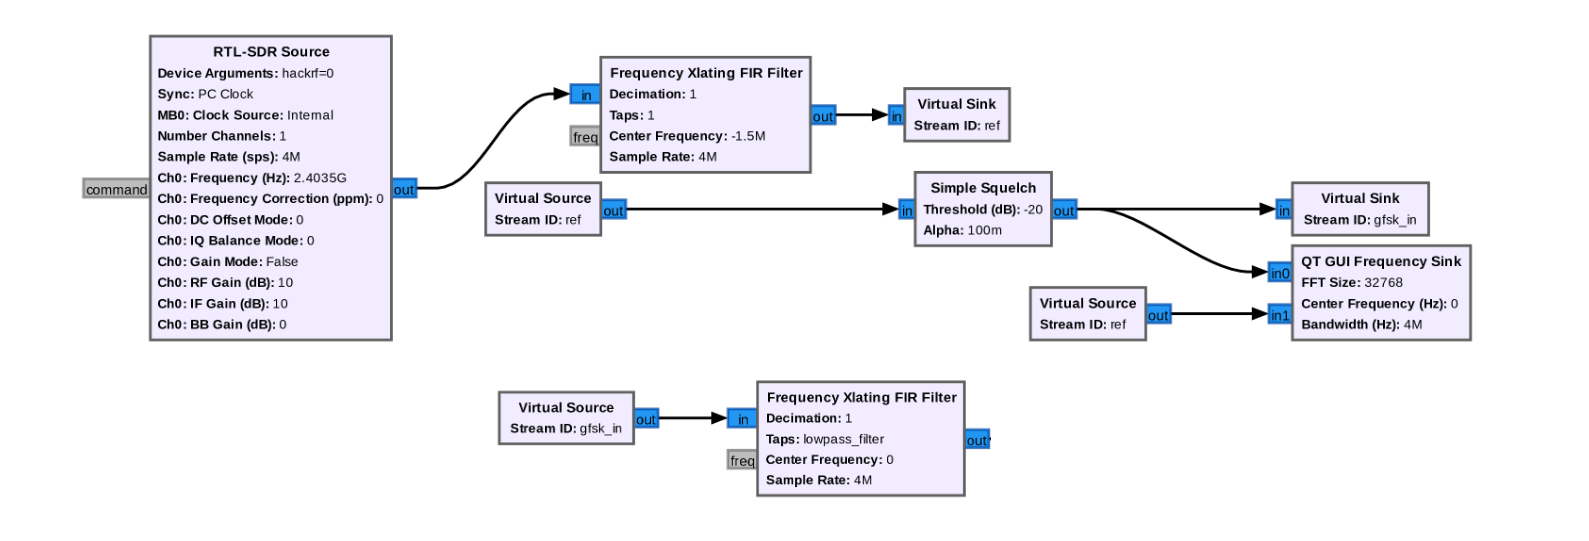
\includegraphics{static/ble-rx-filt.png}
\caption{GNU Radio - Réception et filtrage}
\end{figure}

Sous GNU Radio, le bloc \texttt{RTL-SDR\ Source} va permettre de
recevoir le signal BLE. Il est réglé avec une fréquence
\(f = 2.0435 \ GHz\), et une fréquence d'échantillonnage
\(f_e = 4 \ MHz\). Le décalage fréquentiel pour recentrer le signal est
opéré par le bloc \texttt{Frequency\ Xlating\ FIR\ Filter}, et un
\texttt{Simple\ Squelch} permet de traiter les données uniquement quand
la puissance moyenne est supérieure à -80 dBm, ceci pour éviter d'avoir
trop d'informations.

Enfin, un deuxième \texttt{Frequency\ Xlating\ FIR\ Filter} va servir
cette fois de filtre passe-bande pour garder l'information sur 2 MHz.

\textbf{Démodulation}

\begin{figure}
\centering
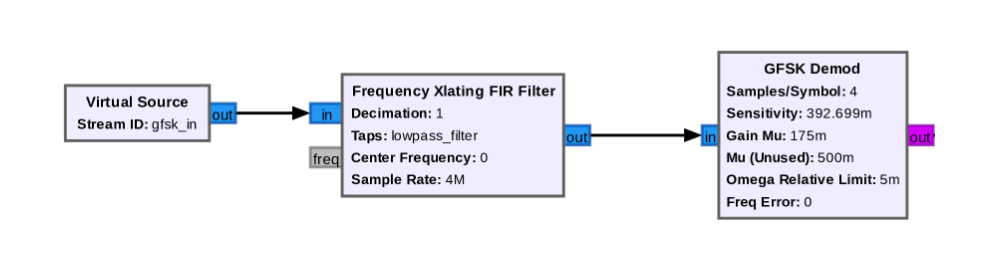
\includegraphics{static/ble-demod.png}
\caption{GNU Radio - Démodulation}
\end{figure}

Le Core v5.3 décrit les paramètres principaux de la modulation GFSK.
Supposant un signal message \(m\) à transmettre, sur une fréquence
\(f_m\) et d'amplitude \(A_m\), ainsi que le signal modulé \(s_{FM}\) à
une fréquence \(f_c\) et une amplitude \(A_c\). Il vient alors :

\[\begin{align}
{m(t) = A_m cos(2 \pi f_m t)} \\
{s_{FM}(t) = A_c cos[2\pi f_c t + \beta_f sin(2 \pi f_mt)]} \\
{\beta_f = \frac{k_f A_m}{2 \pi f_m}}
\end{align}\]

\(k_f\) est la sensibilité de la modulation, définis par
\(k_ f = \frac{2 \pi \Delta f_{max}}{A_m}\).

À noter que si \(\beta_f\) \textless\textless{} 1, la modulation est
appelée Narrow Band Frequency Modulation (NBFM), et pour (\(\beta_f\)
\textgreater{} 1) elle est appelée Wideband Frequency Modulation (WBFM).

Pour démoduler le signal, il va falloir une boucle à verrouillage de
phase, mais elle ne sera pas étudiée ici. Il existe en effet un bloc
\texttt{GFSK\ Demod}, lui-même composé de trois autres blocs : un
\texttt{Quadrature\ Demod}, un \texttt{Symbol\ Sync} et un
\texttt{Binary\ Slicer}. Les deux premiers permettent de démoduler en
quadrature (car la modulation fréquentielle est une modulation de phase)
et de synchroniser l'horloge. Le dernier bloc lui permet d'obtenir
uniquement des bits (0 ou 1).

Ici, pour plus de simplicité, ce sera le bloc \texttt{GFSK\ Demod} qui
sera utilisé. Il y a seulement deux variables à changer : le
\texttt{Samples/Symbol}, défini comme le rapport de la fréquence
d'échantillonnage sur le débit symbole :

\[\begin{aligned}
sps = \frac{f_e}{D_s},
\end{aligned}\]

et la \texttt{Sensitivity}, représentant l'écart possible de fréquence
lors de la modulation :

\[\begin{aligned}
s = \frac{\pi}{2} \frac{1}{sps}.
\end{aligned}\]

La synchronisation d'horloge n'est pas étudiée ici, les valeurs sont
celles par défaut. Cela correspond à l'algorithme de Mueller \& Muller.

\textbf{Exportation}

Pour le BLE, l'envoi de donnée commence toujours par le bit de poids
faible. C'est le rôle des deux derniers blocs,
\texttt{Unpacked\ to\ Packed} et \texttt{File\ Sink} permettant
d'obtenir une suite de byte dans un fichier suivant la convention
\emph{Petit Boutiste}.

Pour visualiser la réception (et donc voir quand une trame Bluetooth est
reçu), un bloc \texttt{QT\ GUI\ Frequency\ Sink} permettra de voir le
spectre du signal en temps réel ainsi que le signal retenu (\emph{i.e.}
quand sa valeur moyenne est à plus de -80 dBm), et un bloc
\texttt{QT\ GUI\ Time\ Sink} permet de voir les bits.

\begin{figure}
\centering
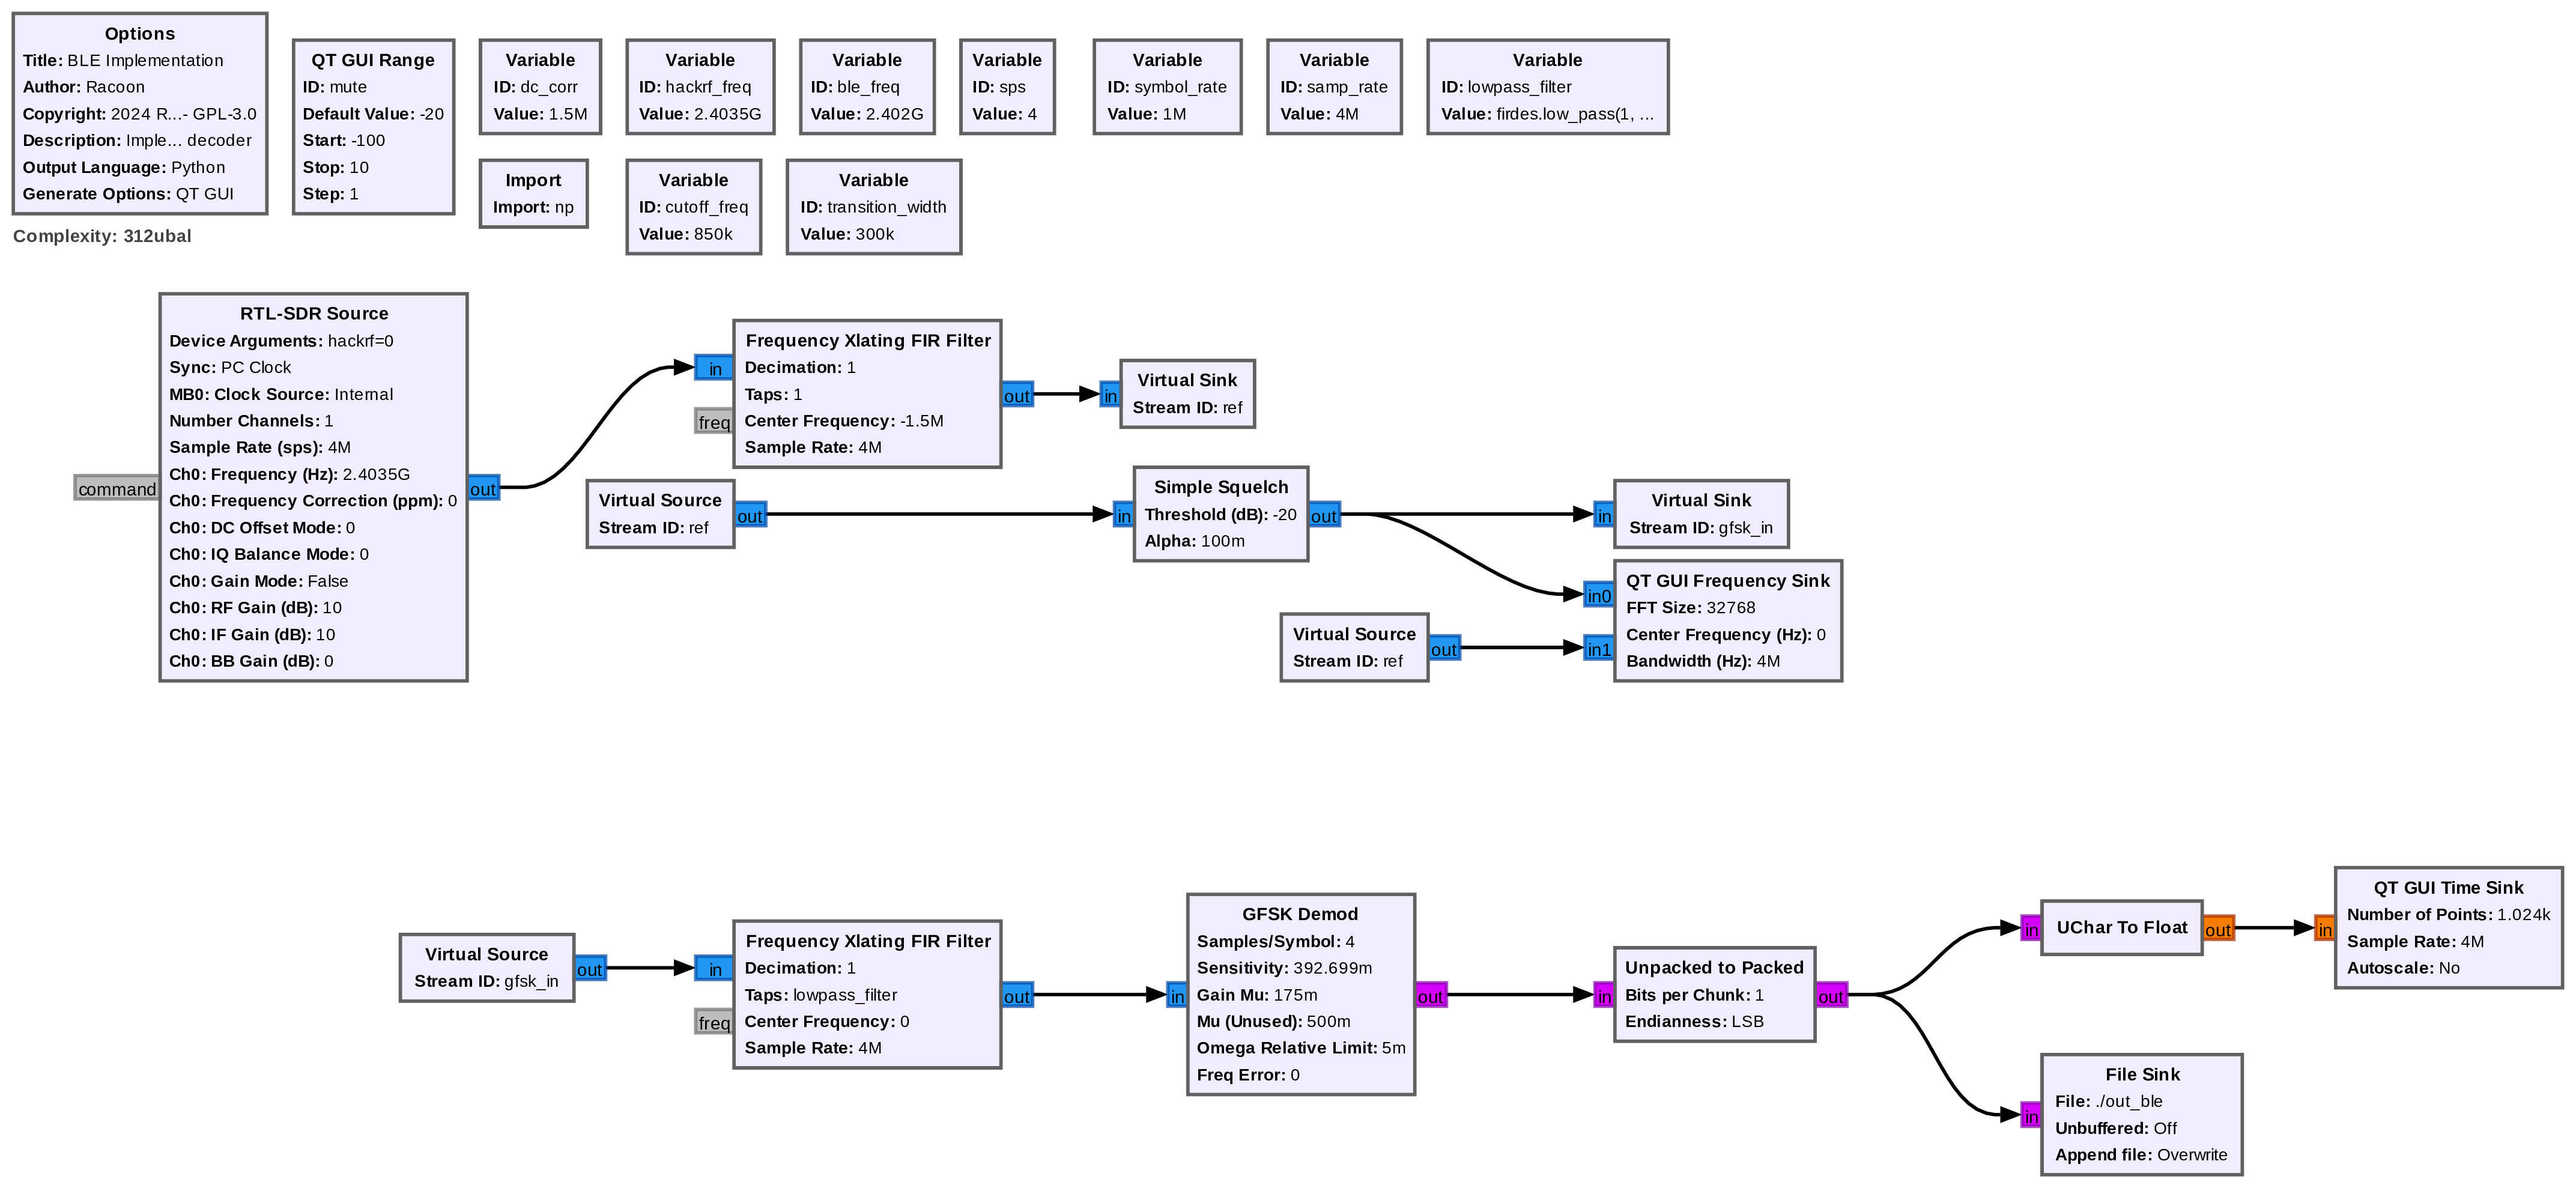
\includegraphics{static/ble-flowgraph.png}
\caption{GNU Radio - Flowgraph complet}
\end{figure}

\subsubsection{3. Python}\label{python}

Maintenant que le signal Bluetooth Low Energy est démodulé, il faut
désormais le décoder. Pour rappel, un ESP 32 émet en continu sur le
canal 37 Advertising, et le graphe GNU Radio a permis de démoduler le
signal, en écrivant les bytes dans un fichier.

Le code \texttt{main.py} est composé de fonctions utiles pour le
décodage et de la classe \texttt{BLEDecode} qui reprend la documentation
\texttt{Bluetooth\ Core\ Specification\ v5.3} étape par étape. L'étude
est restreinte aux trames avec les conditions suivantes :

\begin{itemize}
\tightlist
\item
  La trame est dans le canal 37 Advertising ;
\item
  La transmission suit la variante LE 1M PHY (données non codées, débit
  1 Mb/s).
\end{itemize}

Une trame est définie ainsi :

\begin{figure}
\centering
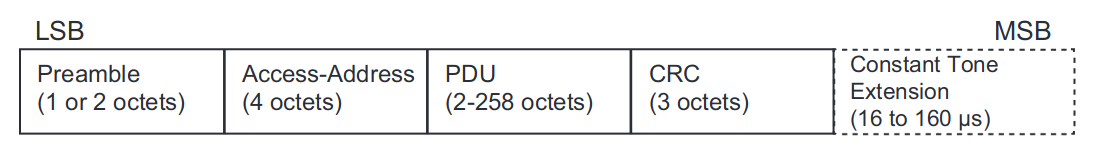
\includegraphics{static/trame.png}
\caption{Trame LE 1M PHY}
\end{figure}

\textbf{Preamble} La trame doit commencer par un octet valant
\texttt{0b10101010}, soit \texttt{\textbackslash{}xAA}\footnote{Bluetooth
  Core Specification v5.3, Vol. 6, Part B, 2.1.1}. Le code python va
donc parcourir l'ensemble du fichier et mettre dans une liste
\texttt{position\_index} l'index de chaque occurence de
\texttt{\textbackslash{}xAA}.

Chaque préambule peut être le début d'une trame. Donc chaque index
présent dans la liste \texttt{position\_index} est potentiellement le
début d'une trame. Le code python va parcourir l'ensemble des index et
va vérifier que le contenu est en adéquation avec la documentation. Le
curseur \texttt{pos} est initié avec la valeur inscrite dans
\texttt{position\_index} et va être incrémenté par la taille mentionné
dans la Trame LE 1M PHY.

\textbf{Access Address} Après le préambule vient 4 octets correspondant
à l'\textbf{Access Address}. Dans le cas du canal d'Advertising, il vaut
systèmatiquement \texttt{0x8E89BED6}\footnote{Bluetooth Core
  Specification v5.3, Vol. 6, Part B, 2.1.2}. La fonction
\texttt{swap\_bytes} permet d'inverser les bytes, car le premier
réceptionné est celui de poids faible. Si l'Access Address est
différent, la trame est abandonné et la variable \texttt{pos} prend la
valeur suivante dans la liste \texttt{position\_index}.

\textbf{PDU} Cette partie peut avoir une taille de 2 à 258 octets. Le
PDU est composé de deux éléments: un \textbf{Header} et un
\textbf{Payload}, le premier étant d'une taille de 16 bits (soit 2
octets) et le second d'une taille allant de 1 à 255 octets.

Le Header est décomposé ainsi :

\begin{figure}
\centering
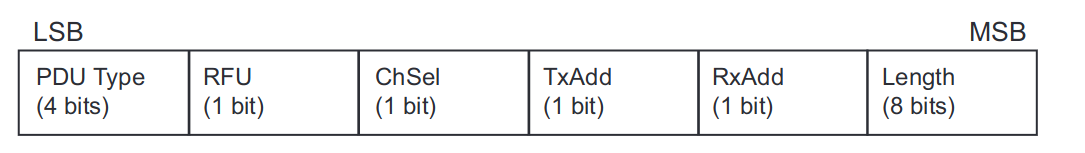
\includegraphics{static/header.png}
\caption{PDU Header BLE}
\end{figure}

Toutefois, pour éviter la répétition de 0 ou de 1 (0b00000000 ou
0b11111111), et donc pour éviter les erreurs, deux algorithmes sont
utilisés:

\begin{itemize}
\tightlist
\item
  Le CRC (vérifier l'intégralité du message) ;
\item
  Le Whitening (éviter les 0 ou les 1).
\end{itemize}

\begin{figure}
\centering
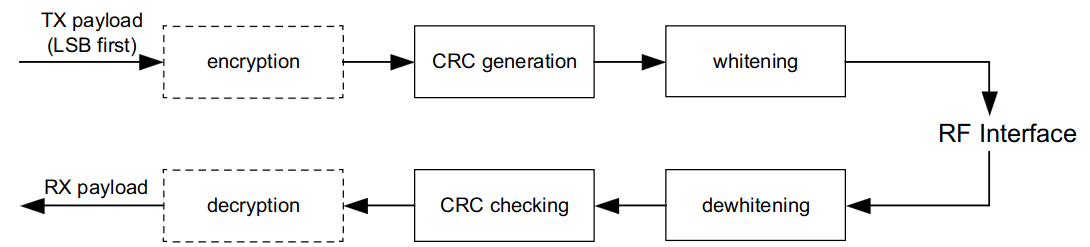
\includegraphics{static/process.png}
\caption{PDU Header BLE}
\end{figure}

Comme l'étude porte sur la réception, il faut d'abord appliquer le
``\emph{dewhitening}''.

\textbf{(De)Whitening} L'algorithme utilise un registre à décalage à
rétroaction linéaire (LFSR).

\begin{figure}
\centering
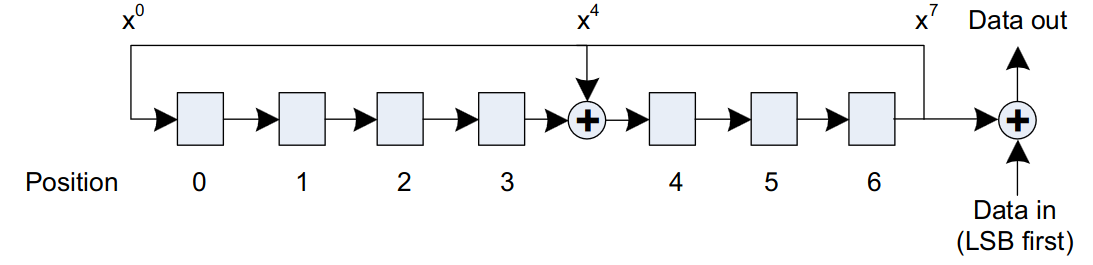
\includegraphics{static/lfsr.png}
\caption{LFSR}
\end{figure}

Le registre est initié ainsi\footnote{Bluetooth Core Specification v5.3,
  Vol. 6, Part B, 3.2}: - La Position 0 prend la valeur 1 ; - Les
Positions 1 à 6 prennent les valeurs du canal en commencant par le bit
de poids fort (les 40 valeurs sont codés sur seulement 6 bits). Ainsi,
pour le canal 37, \(37 |_{10} = 100101|_2\), \(Registre = 110010|_2\).

Le premier bit des données entrante (par exemple, pour `f' dont la
valeur binaire vaut 0b1100110, le premier bit est 0) est xorée avec le
bit de la Position 6. La valeur est ensuite enregistré, et le registre
est décalé d'un cran vers la droite (la valeur en Position 0 passe en
Position 1, etc.). Subtilité : la Position 4 prend la valeur résultante
du XOR entre le bit de la Position 3 et le bit de la Position 6.

A noter : si une valeur est xorée avec 0, sa valeur ne change pas (0
\^{} 0 = 0, 0 \^{} 1 = 1). Au niveau du code Python, cela se traduit
ainsi : - Si le bit à la Position 6 vaut 1, le registre est xorée avec
la valeur 0b10001000. Le registre est alors de taille 8, avec le bit de
poids fort égal à 1, mais l'opération de décalage va enlever le premier
bit et le registre retrouvera une taille valant 7. - Si le bit à la
Position 6 vaut 0, il n'y a pas d'opératoin à faire. La donnée reste
échangé, car elle est xorée avec 0, le bit en Position 4 va prendre
simplement la valeur du bit en Position 3 et le bit de poids fort sera
0.

\textbf{PDU Header} Une fois l'algorithme appliqué sur les données
correspondant au PDU Header, plusieurs valeurs sont mises à dispositions
: - PDU Types ; - RFU ; - ChSel ; - TxAdd ; - RxAdd ; - Payload Length.

Les différents types sont présentés dans la documentation Bluetooth.
\textbar{} PDU Type \textbar{} PDU Name \textbar{} \textbar{} ---
\textbar{} --- \textbar{} \textbar{} 0b0000 \textbar{} ADV\_IND
\textbar{} \textbar{} 0b0001 \textbar{} ADV\_DIRECT\_IND \textbar{}
\textbar{} 0b0010 \textbar{} ADV\_NONCONN\_IND \textbar{} \textbar{}
0b0011 \textbar{} SCAN\_REQ \textbar{} \textbar{} 0b0100 \textbar{}
SCAN\_RSP \textbar{} \textbar{} 0b0101 \textbar{} CONNECT\_IND
\textbar{} \textbar{} 0b0110 \textbar{} ADV\_SCAN\_IND \textbar{}
\textbar{} 0b0111 \textbar{} ADV\_EXT\_IND \textbar{} \textbar{} 0b1000
\textbar{} AUX\_CONNECT\_RSP \textbar{}

La dernière étape est le CRC, permettant de vérifier l'absence d'erreur.
Comme la longueur est désormais connu, la fonction \emph{Whitening} peut
être appliqué au PDU Header, PDU Payload et au CRC. Ce dernier
représente 3 octets, soit 24 bits.

\textbf{CRC} La fonction utilise également un algorithme LFSR. Le
registre est cette fois-ci de 24 bit. Une fois que l'ensemble des
données (PDU Header et PDU Payload) sont passés bit par bit, le registre
aura été décalé X fois, et les 24 bits du registre formeront les 3
octets à comparer avec ceux présent dans la trame.

\begin{figure}
\centering
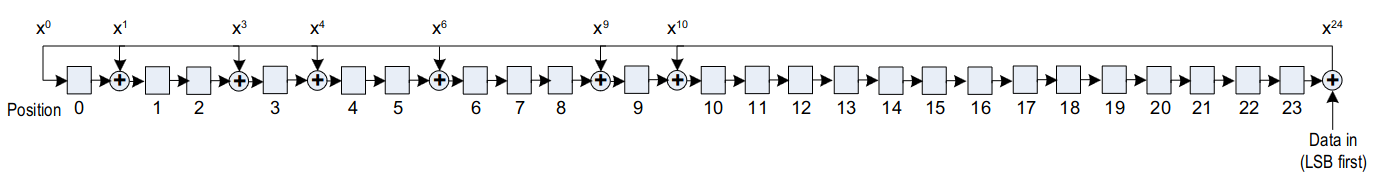
\includegraphics{static/CRC.png}
\caption{CRC}
\end{figure}

Comme la fonction \emph{Whitening}, le décalage se fait par la droite,
et certaines Positions sont xorées avec le bit en Position 24. Le
registre est initialisé avec la valeur 0x555555\footnote{Bluetooth Core
  Specification v5.3, Vol. 6, Part B, 3.1}.

Pour le code Python, si le bit de poids faible (Position 24) à la même
valeur que le bit entrant (celui de la donnée), le bit résultant du XOR
vaudra 0. Le décalage sera simple. Si le bit vaut 1, il faut xoré le
registre avec le bit 0b110110100110000000000000 (correspondant aux
différentes Position où un XOR est nécessaire).

Pour terminer la fonction, les trois bytes sont extraits.

\textbf{Application} Avec le précédent fichier issu de GNU Radio, le
code donne ceci:

\begin{Shaded}
\begin{Highlighting}[]
\ExtensionTok{Access}\NormalTok{ Address found: b}\StringTok{\textquotesingle{}8e89bed6\textquotesingle{}}
\ExtensionTok{PDU}\NormalTok{ Type: ADV\_IND}
\ExtensionTok{CRC}\NormalTok{ correct.}
\ExtensionTok{\{}\StringTok{\textquotesingle{}Access Address\textquotesingle{}}\ExtensionTok{:}\NormalTok{ b}\StringTok{\textquotesingle{}8e89bed6\textquotesingle{}}\NormalTok{, }\StringTok{\textquotesingle{}Type\textquotesingle{}}\NormalTok{: }\StringTok{\textquotesingle{}ADV\_IND\textquotesingle{}}\NormalTok{, }\StringTok{\textquotesingle{}RFU\textquotesingle{}}\NormalTok{: 0, }\StringTok{\textquotesingle{}ChSel\textquotesingle{}}\NormalTok{: 1, }\StringTok{\textquotesingle{}TxAdd\textquotesingle{}}\NormalTok{: 0, }\StringTok{\textquotesingle{}RxAdd\textquotesingle{}}\NormalTok{: 0, }\StringTok{\textquotesingle{}Length\textquotesingle{}}\NormalTok{: 37, }\StringTok{\textquotesingle{}Payload\textquotesingle{}}\NormalTok{: b}\StringTok{\textquotesingle{}\textbackslash{}xc9\textbackslash{}xc8\textbackslash{}xe7\textbackslash{}xa1\textbackslash{}xdf|\textbackslash{}x02\textbackslash{}x01\textbackslash{}x06\textbackslash{}x06\textbackslash{}tESP32\textbackslash{}x02\textbackslash{}n\textbackslash{}t\textbackslash{}x11\textbackslash{}x07K\textbackslash{}x911\textbackslash{}xc3\textbackslash{}xc9\textbackslash{}xc5\textbackslash{}xcc\textbackslash{}x8f\textbackslash{}x9eE\textbackslash{}xb5\textbackslash{}x1f\textbackslash{}x01\textbackslash{}xc2\textbackslash{}xafO\textquotesingle{}}\NormalTok{, }\StringTok{\textquotesingle{}CRC\textquotesingle{}}\NormalTok{: b}\StringTok{\textquotesingle{}eL\textbackslash{}x0b\textquotesingle{}}\NormalTok{, }\StringTok{\textquotesingle{}Address\textquotesingle{}}\NormalTok{: }\StringTok{\textquotesingle{}0x7cdfa1e7c8c9\textquotesingle{}}\NormalTok{\}}
\end{Highlighting}
\end{Shaded}

\section{Conclusion}\label{conclusion}

\section{Technologies utilisées}\label{technologies-utilisuxe9es}

\subsection{GNU Radio}\label{gnu-radio-1}

First flowgraph:

\begin{itemize}
\tightlist
\item
  Input: text file or PDF file.
\item
  Byte stream (unsigned char).
\item
  Packet of 35 bytes with 2 header bytes.
\item
  GFSK modulation.
\end{itemize}

Parameters:

\begin{itemize}
\tightlist
\item
  Sample rate: 1 MHz or 2 MHz
\item
  Frequency deviation: 50 kHz (according to
  \texttt{Bluetooth\ Core\ Specification\ V4.0})
\item
  Modulation index N = frequency\_deviation / sample\_rate
\item
  BT (Gaussian filter bandwith): 0.5 (according to
  \texttt{Bluetooth\ Core\ Specification\ V4.0})
\item
  Samples per symbol: BT / N
\item
  Sensitivity (GFSK block): 2 * pi * frequency\_deviation / sample\_rate
  (according GNU Radio documentation)
\end{itemize}

\section{Conclusion}\label{conclusion-1}
